\documentclass[onecolumn, draftclsnofoot, 10pt, compsoc]{IEEEtran}
\usepackage{graphicx}
\usepackage{url}
\usepackage{setspace}
\usepackage{geometry}
\usepackage{listings}
\usepackage{tikz}
\usetikzlibrary{arrows,automata}
\usepackage{caption}

\geometry{textheight=9.5in, textwidth=7in}

% 1. Fill in these details
\def \CapstoneTeamName{			Team 41}
\def \CapstoneTeamNumber{		41}
\def \GroupName{				30k CS Avionics}
\def \GroupMemberOne{			Joshua Novak}
\def \GroupMemberTwo{			Allison Sladek}
\def \GroupMemberThree{			Levi Willmeth}
\def \CapstoneProjectName{		30K Rocket Spaceport America}
\def \CapstoneSponsorCompany{	Oregon State University}
\def \CapstoneSponsorPerson{	Dr. Nancy Squires}

% 2. Uncomment the appropriate line below so that the document type works
\def \DocType{		%Problem Statement
					%Requirements Document
 					%Technology Review
 					%Preliminary Design Document
					Progress Report
				}
			
\newcommand{\NameSigPair}[1]{
	\par
	\makebox[2.75in][r]{#1} \hfill
	\makebox[3.25in]{\makebox[2.25in]{\hrulefill} \hfill \makebox[.75in]{\hrulefill}}
	\par\vspace{-12pt}
	\textit{
		\tiny\noindent \makebox[2.75in]{} \hfill
		\makebox[3.25in]{\makebox[2.25in][r]{Signature} \hfill \makebox[.75in][r]{Date}}
	}
}
% 3. If the document is not to be signed, uncomment the RENEWcommand below
%\renewcommand{\NameSigPair}[1]{#1}
% \renewcommand{\thesubsubsection}{\thesection.\alph{subsubsection}}

%%%%%%%%%%%%%%%%%%%%%%%%%%%%%%%%%%%%%%%
\begin{document}
\begin{titlepage}
    \pagenumbering{gobble}
    \begin{singlespace}
    	%\includegraphics[height=4cm]{coe_v_spot1}
        \hfill 
        % 4. If you have a logo, use this includegraphics command to put it on the coversheet.
        %\includegraphics[height=4cm]{CompanyLogo}   
        \par\vspace{.2in}
        \centering
        \scshape{
            \huge CS Capstone \DocType \par
            {\large\today}\par
            \vspace{.5in}
            \textbf{\Huge\CapstoneProjectName}\par
            \vfill
%             {\large Prepared for}\par
%             \Huge \CapstoneSponsorCompany\par
%             \vspace{5pt}
%             {\Large\NameSigPair{\CapstoneSponsorPerson}\par}
            {\large Prepared by }\par
%            	\GroupName\par
            % 5. comment out the line below this one if you do not wish to name your team
%             \CapstoneTeamName\par
            \vspace{5pt}
            {\Large
                \NameSigPair{\GroupMemberOne}\par
                \NameSigPair{\GroupMemberTwo}\par
                \NameSigPair{\GroupMemberThree}\par
            }
            \vspace{20pt}
        }
    \end{singlespace}
    
    \section*{Revision History}
    \begin{tabular*}{1\linewidth}{@{\extracolsep{\fill}}|c|c|c|c|}
      \hline
      Name & Date & Reason For Changes & Version\\
      \hline
      Levi Willmeth, Joshua Novak, Allison Sladek&11/28/17&Initial document draft&0.1\\
      \hline
    \end{tabular*}
	\\
    
    \begin{abstract}
    Progress report document outlining Team 41's goals, progress, and challenges during Fall semester of our Computer Science Capstone class while working on Oregon State University's 2017-18 entry to the Spaceport America Cup.
	\end{abstract}
\end{titlepage}
\newpage

\pagenumbering{arabic}

\tableofcontents
% 7. uncomment this (if applicable). Consider adding a page break.
%\listoffigures
%\listoftables

%===============================================================================
%Start Problem Statement w/o Metrics
\newpage
\section{Project Overview}
This computer science (CS) capstone project will include writing software to support the Oregon State University (OSU) American Institute of Aeronautics and Astronautics (AIAA) team's entry for the Spaceport America Cup 30k competition in the summer of 2018.  The competition involves designing, building, and launching a student-made rocket to 30,000 feet.

%===============================================================================

\section{Problem Definition}
Our goals for entering the Spaceport America Cup are to learn and experience working together as a team to build a rocket, and to also score highly during the competition.  As such, the scoring criteria are very important to forming the needs of our project.  The exact scoring metric has not been released yet, but we expect the software components will include avionics to control the rocket, receiving near real time telemetry on the ground during the flight, and visualizing the results of an onboard scientific payload after the flight.  Our task will be to write the software necessary to accomplish those goals.

The AIAA team includes several sub teams that will all need to work together.  In particular, we will need to work with the electrical and computer engineering (ECE) students who are responsible for developing the avionics hardware and telemetry radio systems.  The ECE subteam is ultimately responsible for those systems, but we will provide support to write the necessary software.  It is important to support the overall team because at the competition we will all succeed or fail together.

Our subteam will focus on designing a ground system capable of collecting and viewing flight data, and programs to control flight avionics for the rocket and scientific payload.

%===============================================================================

\section{Proposed Designs and Solutions}

\subsection{Ground Station}

\begin{center}
	\includegraphics[width=0.5\textwidth]{images/parser_diagram.eps}
    \label{parser-diagram}
    \captionof{figure}{Flow of information through the ground station.}
\end{center}

We are building a ground station program to receive, parse, store, and serve all of the data recorded during the rocket's flight.  This information will be available to users over a web page served over local WiFi.

The ground station will be contained in a hard travel box for ease of transportation and to protect the delicate electrical components in the harsh desert environment of the New Mexico desert, where the final competition will be held.

The ground station will contain four Raspberry Pi micro computers, a Raspberry Pi 3B, a battery with USB outputs, and a small screen used for debugging problems.  It will serve an ad-hoc WiFi network to allow nearby users to view flight data using their cell phones, tablets, or laptops.

\subsection{Networking}
The Raspberry Pi 3B computer in the ground station will be serving a local WiFi network that nearby people can join to interact with our system.  Each of the Raspberry Pi Zero computers will be networked to the main Pi 3B computer using USB OTG, which allow them to be powered and networked over a single USB cable.  We will be able to ssh into the Pi 3B or Pi Zeros using this WiFI network.

\subsection{Displaying the Data}
The Raspberry Pi 3B computer will be serving a web page to computers that are connected to it's WiFi network.  The web page will pull data from the Pi 3B's database and display dynamic and static graphs and information in relevant ways.  The system will allow users to view static data from previous flights, or dynamic data from active flights.  The primary interface for this information will be an HTML page that can be viewed using cell phones, tablets, and laptop computers.

\subsection{Data Parser}
We are designing a parsing program that will run on each of the four Raspberry Pi Zero computers inside the ground station.  The parsing program will take in a file of raw sensor values from the onboard electronics, or an audio source for live telemetry data from a hand held radio.  The program will validate telemetry data using a checksum, or file data by comparing expected fields.  It will then write the information into a database on the same network.

\begin{center}
	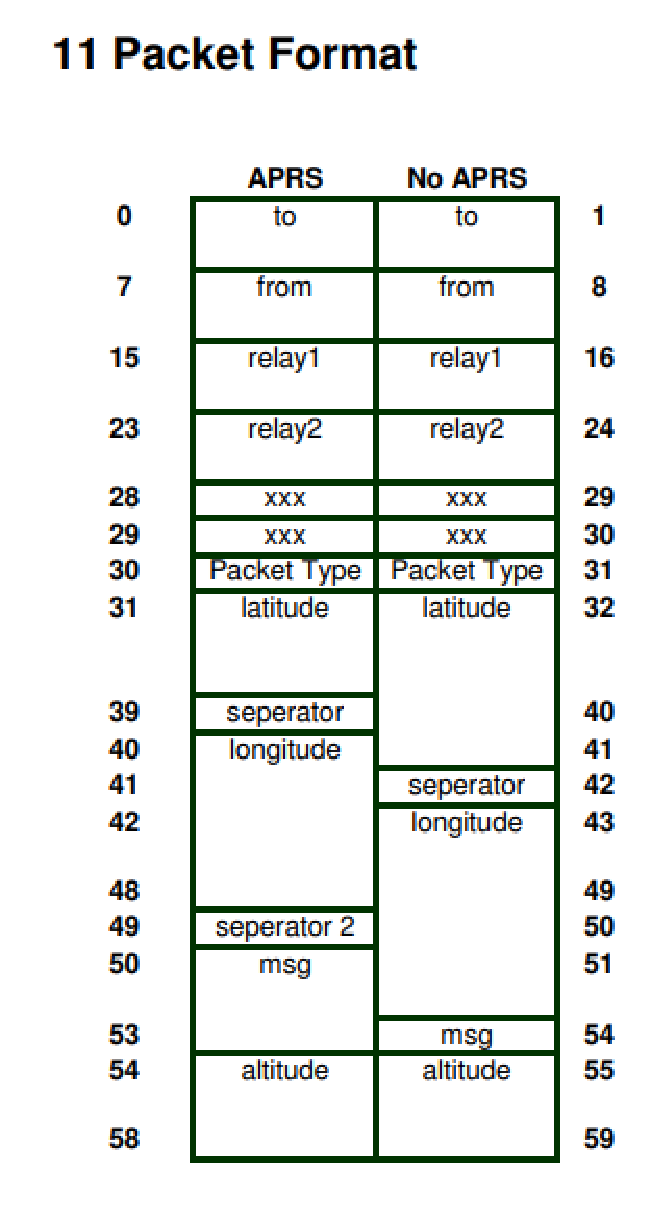
\includegraphics[width=0.2\textwidth]{images/beelinegps-packet-format.eps}
    \label{parser-diagram}
    \captionof{figure}{Format of BigRedBee BeelineGPS APRS telemetry packets.}
\end{center}

\subsection{Database}
The database will be served by a Raspberry Pi 3B computer in the ground station.  The database will collect and store all data recorded during the flight, and relate records inserted at different times and from different sources by using a combination of primary and foreign keys. This will allow the website to select records based on a given flight, or range of time, even though the records will be stored across several tables.

\begin{center}
	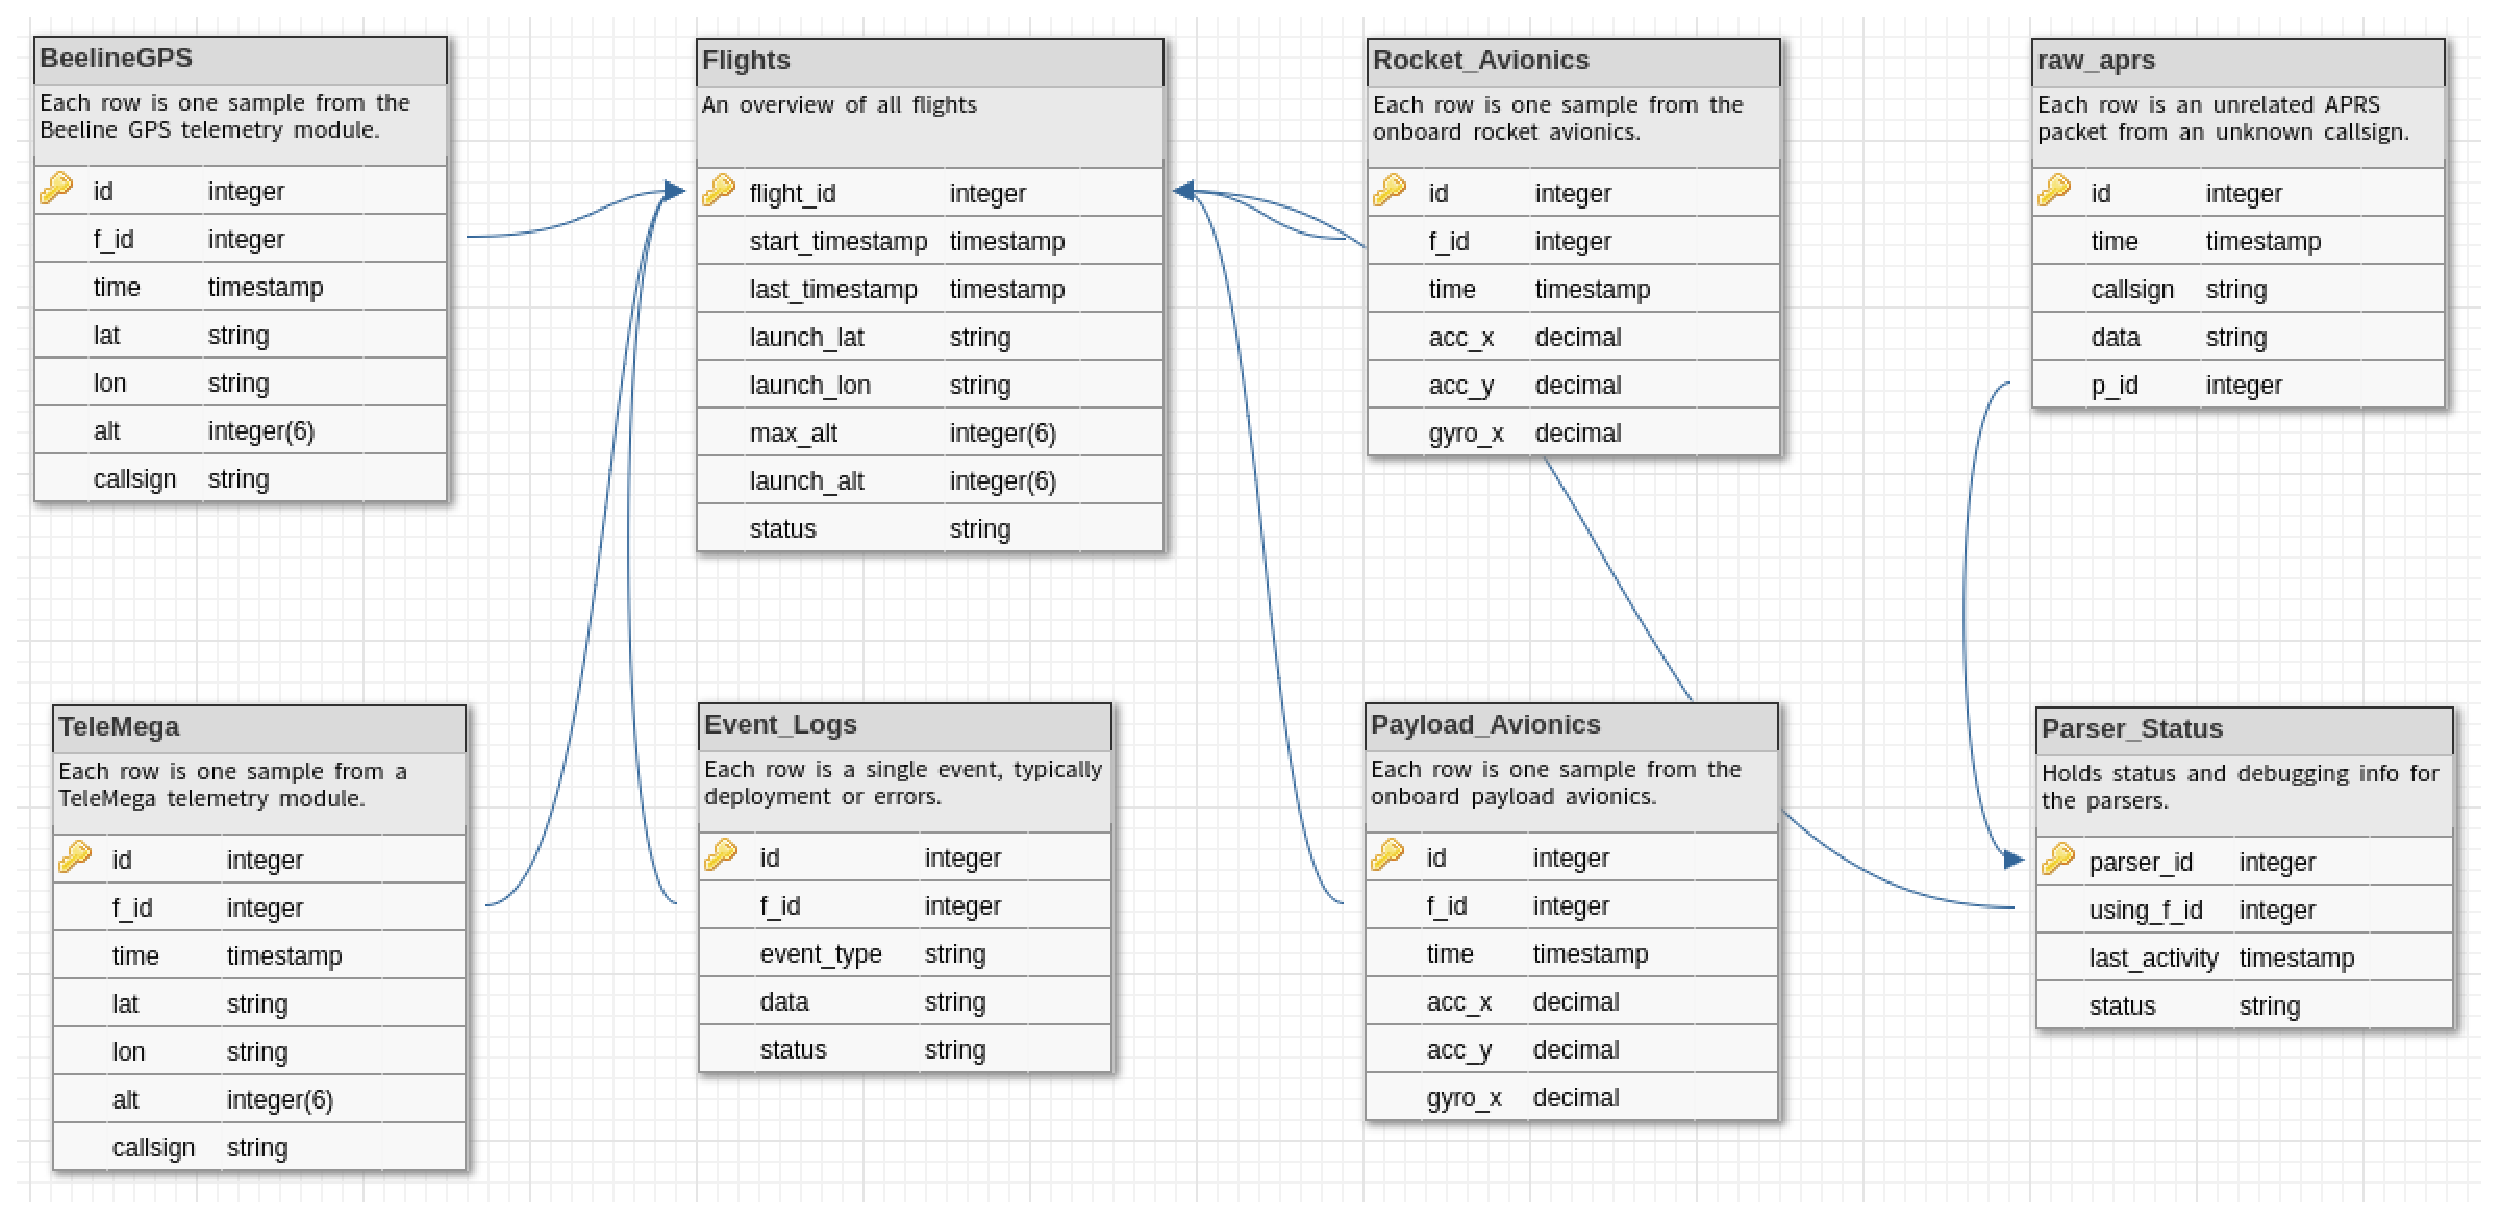
\includegraphics[width=\textwidth]{images/database_schema_v102.eps}
    \label{database-schema}
    \captionof{figure}{Early draft of the database schema.}
\end{center}

\subsection{Avionics Software}

The rocket will contain two flight computers, one of which will remain with the body of the rocket while the other will be ejected at apogee with the scientific payload.

The flight computer that remains inside the body of the rocket will be running a program we call the Rocket Avionics.  The flight computer inside the payload will be running the Payload Avionics.

\subsubsection{Rocket Avionics}
The Rocket Avionics have two primary goals: accurately detect apogee and trigger separation, and record data from onboard sensors to an SD card for later analysis.

Apogee will be detected using a combination of onboard accelerometers, gyroscopes, barometers, and Kalman filters to ignore erroneous data.  This is a mission-critical task as early separation would destroy the rocket, and late separation would prevent the scientific payload from successfully completing it's mission.

Storing data onto the SD card is a secondary task that will be performed as quickly as possible.  The goal here is to record as many samples as possible, while giving CPU priority to the task of detecting apogee.

\subsubsection{Payload Avionics}
The Payload Avionics will also perform two primary goals: using a propeller to push the payload towards the ground at the correct rate in order to neutralize gravity, and recording data from onboard sensors to an SD card for later analysis.

The scientific experiment will be attempting to achieve zero gravity for 10-12 seconds.  Accomplishing that will require spinning the propeller slowly at first because the payload will begin falling at nearly the $9.82 m/s^2$ as gravity.  However, as the payload's velocity increases, the force of drag will increase and the propeller will become less effective, necessitating an increased amount of thrust.  We will use an array of three accelerometers and gyroscopes to measure the current acceleration, and a closed PID loop to dynamically calculate the speed to spin the motor to either increase or decrease the payload's acceleration with the goal of achieving zero acceleration from the perspective of the payload.

Simultaneously, the payload will be logging these sensor values onto an SD card in order to measure the success of our stated goal of achieving zero gravity.

%===============================================================================

\section{Support the AIAA team as a whole}
Another goal for this project is to support the entire team, not just the computer science subteam.  To do our part, we will attend regular team meetings and try to understand the problems and challenges faced by the other subteams.  If we see an opportunity to help another subteam with something, we will do our best to do so.  We will also attend the majority of team building and training exercises, as well as all practice rocket launches.

Sometimes, supporting the rest of the team means asking for help from them.  In the event that we are the ones who need support, we will talk with our team members and ask for help.  We will stay in communication with our primary sponsor Dr. Nancy Squires, and other team mentors.  We will treat ourselves and other team members with respect, and do our best to create a good working environment both online and in person.

%===============================================================================

\section{Moving Forward}
We plan to work on the GUI over Winter Break, ideally having the server, database, website, and graphs finished by the end of the break. This will leave us to work on the avionics over the term alongside the test suites, which will allow us to more easily work alongside the other sub-teams. Also, it will mean that if adjustments need to be made for one reason or another, we will have plenty of time to do so. The other reason that we will be working on these elements over Winter break is that they are the least reliant on the input or needs of other groups, so we won't need to communicate with anyone outside of our own team to complete them. They are also the least reliant on input from our TA since the choices we made for these elements make them fairly straight-forward and should not require too much assistance or advice from the TA.

%===============================================================================

\section{Weekly Overview}

%This table can be moved somewhere else in the document.
\begin{tabular}{ | p{0.1\linewidth} | p{0.25\linewidth} | p{0.25\linewidth} | p{0.25\linewidth} | }
\hline
&
Summary&
Problems&
Solutions\\\hline
Week 1&
First ERSA meeting, Allison and Joshua did not attend as they were not yet members of the team. OneNotes setup, bids made.&
&\\\hline
Week 2&
Problem statement rough drafts started, group formed.  We met with Nancy on Friday to outline the problem statement.&
The problem requirements were somewhat vague, we needed to meet with other sub-teams in order to understand the project.&
We spoke with the ECE team multiple times throughout the term in order to understand what our role was with the project, and attended regular ERSA meetings for the same reason.\\\hline

Week 3&
Rough drafts of problem statement submitted
Met with the ECE team to understand what our respective responsibilities were.
Met with our TA, who outlined how our work will be graded and gave us recommendations on how to interact with the client.
There was a meeting between the 100k team and their peer mentor, which Levi attended and learned a lot from.&
&\\\hline

Week 4&
We started looking for code from the previous year’s CS team, as well as their ground station.
Finished problem statement and had it approved by Nancy.&
We ran into a lot of trouble finding the code from the previous year. The Google Drive folder for the previous year only had the ECE team’s code, and most people we reached out to were unable to help.&
Ryan from last year’s ECE team attended the meeting during week 9, and he was able to show us the previous year’s ground station and linked us to their code. By this point we had already come up with our own design though.\\\hline
\end{tabular}

% This was split into two tables because one was too long for a single page
\newpage
\begin{tabular}{ | p{0.1\linewidth} | p{0.25\linewidth} | p{0.25\linewidth} | p{0.25\linewidth} | }
\hline
&
Summary&
Problems&
Solutions\\\hline

Week 5&
We started the requirements document.
We found CanvasJS, an option for our GUI that would allow us to display the ground station through a web page. This was ultimately the option we went with for the GUI.&
The ECE team’s choice of telemetry unit severely limited the range of fields that we could expect to receive to display with the GUI, specifically it only transmits GPS, altitude, and a timestamp.&
We did research to show that a different telemetry unit would not have significant negative tradeoffs, but the ECE team was not persuaded. Ultimately we decided to create our GUI such that it would be able to display those fields if they were available, and will create a test to demonstrate this.\\\hline

Week 6&
We started dividing up the sections for our Tech Review during this week, and turned in the Technical Requirements document.&
&\\\hline

Week 7&
During this week we finished dividing our Tech Review up. We also started researching the various technologies we planned to use.&
&\\\hline

Week 8&
We continued the Tech Review, with each of us researching our different areas.&
We discovered there may be a licensing issue with CanvasJS.&
We emailed the sales team for the product, and learned that our project could use a non-commercial version of the product.\\\hline

Week 9&
Learned that ECE team will be able to write their own separate code to satisfy their requirements.
We finished and submitted our Tech Reviews.
We started dividing up responsibilities for the design document.&
The ECE team was told by one of their mentors that they had to use a hardware solution for triggering flight events. This means that our avionics will ultimately be non-functional.&
We will write code that can determine when flight events should be triggered and will record them, alongside when the hardware determines that flight events should be triggered.
Going forward we will do more to reach out to the ECE team to ensure that information like this reaches us sooner.\\\hline

Week 10&
Worked on Design Document and Progress Report.&
&Nancy Squires approved using last year's Altus Metrum telemetry module (or purchasing a new one) for our display during Spring Expo.
\\\hline
\end{tabular}

%===============================================================================

%Start of Retrospective Table
\newpage
\section{Retrospective}
\begin{tabular}{ | p{0.3\linewidth} | p{0.3\linewidth} | p{0.3\linewidth} | }
\hline
Positives&
Deltas&
Actions\\\hline
Finding CanvasJS gave us a method to create our graphs quickly and effectively.&
We need to communicate with the ECE team better and more regularly.&
We will reach out to them on their slack channel more regularly, and occasionally arrange meetings with them on weeks where we don’t have a general meeting.\\\hline

Nancy has been very easy to work with, as have the different sub-teams.&
We need a HAM radio license.&
One of us get one of these licenses, likely Allison since she has expressed interest in this in the past.\\\hline

We were able to get access to a Raspberry Pi for testing.&
We do not have sensors for testing and will need those moving forward.&
We will get some spare sensors from the ECE team to use for testing purposes.\\\hline

The ECE team decided to use a Raspberry Pi as the computer on both the rocket and the payload, making coding much easier.&
We currently do not have the hardware for our ground station and will need to acquire that.&
We will order some of this hardware with our part of the budget. Some of the hardware, such as Raspberry Pi’s, may be able to be acquired from Kevin, and one has been borrowed for testing purposes.\\\hline

Due to the required AIAA membership and variety of mentors working with the team, we have had many opportunities to expand our knowledge of rocketry.&
We need to decide on how we want to structure our avionics code.&
We will do tests with a few sensors and different methods of writing the avionics code either over winter break or early in the term.\\\hline

It has been very interesting working with engineering students outside of CS.&&\\\hline
\end{tabular}

%========================================================================================End of Problem Statement w/o Metrics

%========================================================================================Chart from Requirements

\newpage
%\begin{figure}
%	\centering
%    Dependencies Flowchart
%	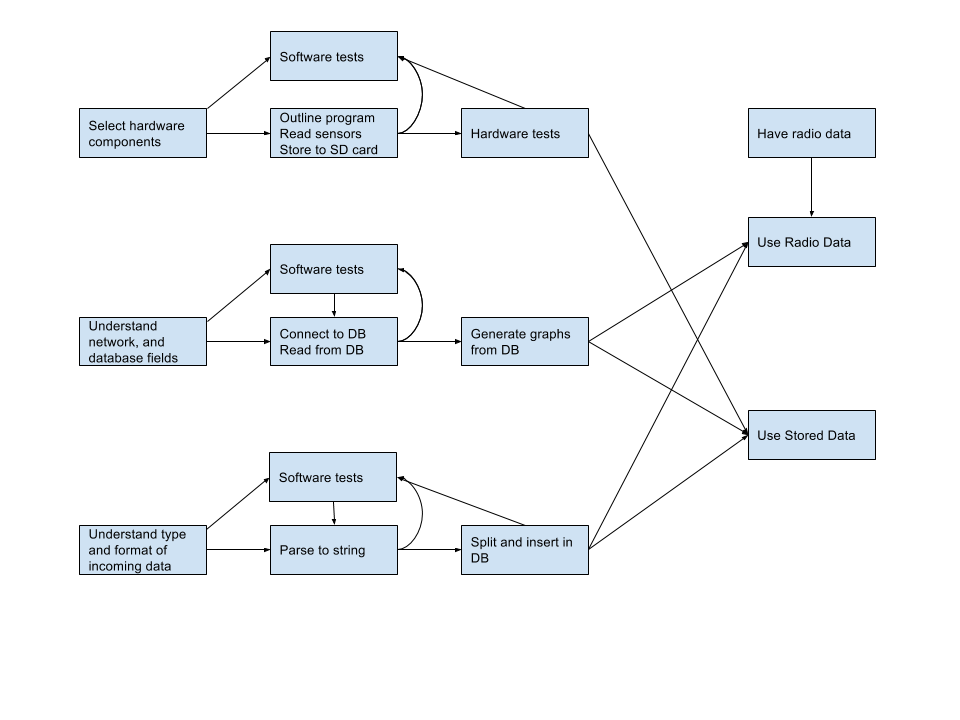
\includegraphics[scale=0.5\textwidth, natwidth=960, natheight=720]{dep_flowchart.png}
%\end{figure}
%======================================================================End of Flow Chart
\end{document}
